\documentclass{standalone}
\usepackage{tikz,pgfplots,calc,tkz-euclide}
\usetikzlibrary{positioning,calc}
\usetikzlibrary{arrows}
\usepackage{tkz-euclide}
\usetkzobj{all}


\begin{document}
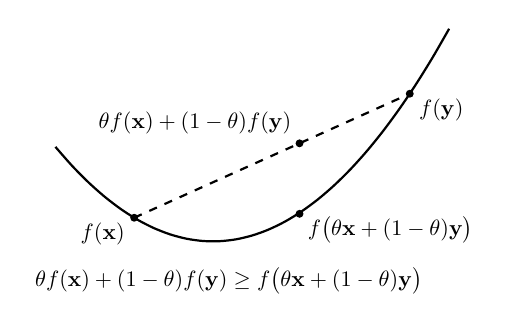
\begin{tikzpicture}[>=stealth, thick]
   
    \def\a{1}
    % \begin{scope}[xshift = 14cm, yshift = -3cm, scale = 1.7]
        % \draw[domain=-2:1.5,smooth,variable=\x,black] plot ({\x},{exp(\a*\x)});      
        \draw[domain=-2:3,smooth,variable=\x,black] plot ({\x},{.3*\x*\x});  


        \def\xx{-1}
        \def\xy{.3}    
        \def\yx{2.5}
        \def\yy{6.25*.3}
        \def\t{.4}
        \def\u{.6}
        \def\zx{{\t*\xx + \u*\yx}}
        \def\zx{1.1}
        \def\zy{{\t*\xy + \u*\yy}}
        \def\vy{{.3*\zx*\zx}}
        \def\vy{.35}

        \draw [fill = black, draw = black] (\xx, \xy ) circle (1pt);
        \draw [fill = black, draw = black] (\yx, \yy ) circle (1pt);
        \draw [fill = black, draw = black] (\zx, \zy ) circle (1pt);
        \draw [fill = black, draw = black] (\zx, \vy ) circle (1pt);
        \draw [dashed] (\xx, \xy) -- (\yx, \yy);

        % \draw [dashed] (\xx, \xy) -- node[left] {$\theta f(\mathbf{x}) + (1 - \theta)f(\mathbf{y})$} (\yx, \yy);

        \node [scale = .8] at (\xx - .4, \xy - .2) {$f(\mathbf{x})$};
        \node [scale = .8] at (\yx + .4, \yy - .2) {$f(\mathbf{y})$};
        \node [scale = .8, anchor = west] at (\zx, \vy - .2) {$f\big(\theta\mathbf{x} + (1 - \theta)\mathbf{y}\big)$};

        \node [scale = .8, anchor = east] at (\zx, 1.5) {$\theta f(\mathbf{x}) + (1 -\theta) f(\mathbf{y})$};
        \node [scale = .8] at (0.2, -.5) {$\theta f(\mathbf{x}) + (1 -\theta) f(\mathbf{y}) \geq f\big(\theta\mathbf{x} + (1 - \theta)\mathbf{y}\big)$};



        % \node [scale = 2] at (1, 4) {$f(x) = \frac{1}{2}(x-1)^2 - 2$};
        % \foreach \xx in {.1}{
        %     % \draw [fill = black] (\xx, {.5*(\xx - 1)^2 - 2}) circle (1pt);
        %     \draw[->, red, thick, domain=(\xx-1):(\xx+1),smooth,variable=\x] plot ({\x},{(\a*exp(\a*\xx))*(\x - \xx) + exp(\a*\xx)});      
        % }

        % % \

        % \def\x{.1}
        % \def\xp{1.2}
        % \def\xm{-1}
        % \def\y{{exp(\a*\x)}}
        % \def\yp{{exp(\a*\xp)}}
        % \def\ym{{exp(\a*\xm)}}

        % \draw [->, green!80!black] (\xm, \ym) -- (\x, \y);
        % \draw [->, blue] (\x, \y) -- (\xp, \yp);
        % \draw [->, orange!80!black] (\xm, \ym) -- (\xp, \yp);

        % \draw [dashed] (\xm, \ym) -- node[below] {$\varepsilon$} (\x, \ym);
        % \draw [dashed] (\x, \y) -- node[above] {$\varepsilon$} (\xp, \y);
        % \draw [dashed] (\x, \ym) -- node[right]{$f(x_0) - f(x_0 - \varepsilon)$} (\x, \y);
        % % \draw [dashed] (\xp, \y) -- (\xp, \yp);
        % \draw [dashed] (\xp, \y) -- node[right]{$f(x_0 + \varepsilon) - f(x_0)$} (\xp, \yp);


        % \draw [dashed] (\xm, \ym) -- node[left]{$f(x_0 + \varepsilon) - f(x_0 - \varepsilon)$} (\xm, \yp);
        % \draw [dashed] (\xm, \yp) -- node[above]{$2\varepsilon$} (\xp, \yp);
% 
        % \draw ()
        % \draw [fill = black, draw = black] (\x, \y ) circle (1pt);
        % \draw [fill = black, draw = black] (\xp, \yp) circle (1pt);
        % \draw [fill = black, draw = black] (\xm, \ym) circle (1pt);
        % \draw [fill = black, draw = black] (\x, \ym) circle (1pt);
        % \draw [fill = black, draw = black] (\xm, \yp) circle (1pt);
        % \draw [fill = black, draw = black] (\xp, \y) circle (1pt);


        % \node [scale = 3] at (1, -1.5) {$x^*$};
    % \end{scope}

    % \draw[domain=-3:-2] plot (\x,{(\x-1)*(\x-1)-2}) {[turn] (-3,) coordinate(t1) (-1,0) coordinate(t2)};
    % \draw[domain=-2:2] plot (\x,{(\x-1)*(\x-1)-2});
    % \draw[red] (t1)--(t2);


\end{tikzpicture}
\end{document}